
\chapter{Method}

In this section, we will talk about the methodical part of our work. Part of this is to establish preliminaries, explain how we prepared our data, and finally how we structured our visualization. For the concrete technical details, we refer to \ref{imp}.
% %%%%%%%%%%%%%%%%%%%%%%%%%%%%%%%%%%%%%%%%%%%%%%%%%%%%%%%%%%%%%%%%%%%%%%%%
\section{Preliminaries}
Microblogging services are platforms, where users can post messages for other users to read. Messages are most often capped in their length and visible for anyone to see. Users can choose to follow each other, meaning that they will be updated when the person they are following has posted anything new, and search for content by filtering, using \emph{hashtags}, which are keywords which can be added to any message, to mark its relevance to the keyword. 

\emph{Twitter} allows responding to posts publicly, which is called \emph{retweeting}. Users can see the new message, as well as the post it is referencing. We call any chain of post-responses a \emph{thread}.
\section{Data Preparation}


The basic element through which all discourse is organized in our tool is the message. A single message must contain following information:
\begin{itemize}
    \item message text
    \item message author
    \item location sent
    \item time sent
\end{itemize}
Optionally following information can be contained:
\begin{itemize}
    \item message to which current message is answer
    \item number of interactions by other users
    \item any additional dimension an user might be interested in
\end{itemize}

\begin{figure}
  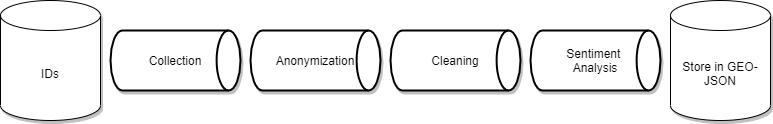
\includegraphics[width=\linewidth]{figures/data pipeline.png}
  \caption{A visualization of the pipeline, which we used for the pre-processing of our data}
  \label{fig:viz2}
\end{figure}
\label{data_prep}

Most microblogging services like \emph{Twitter} provide an API for data collection in combination with their policies.
To ensure integrity and safety of users data, firstly, the message authors have to be anonymized in such a way that no user could be identified via the dataset. Afterwards, additional preparation steps can be taken to prepare the data for analytical purposes. We will lay out the steps we took in our example, but explore additional possibilities later on. 

Our pipeline consists of following steps: Data collection, data anonymization, textual cleaning, sentiment analysis and data storage.
Data collection is done via the official Twitter API\footnote{\url{https://developer.twitter.com/en/docs/tools-and-libraries}} for Python, through which tweets can be selected by ID. We chose to focus on messages which talked about the COVID-19 pandemic, a dataset for which is provided by ~\cite{DVN/LW0BTB_2020}. After receiving the tweets through the API, the authors were replaced by randomized IDs, which were stored together with the message texts, IDs of targets, location and timestamp. Messages without any location or timestamp were removed, since they could not be visualized reasonably. 

To clean the textual data, we lower cased all letters and removed punctuation as well as special characters like emojis. This cleaned version is only used for the sentiment analysis later on. When showing the text to the user, we still use the original version. 

In our example, we chose to apply a sentiment analysis to the message texts, to show one additional dimension. Tools and resources for sentiment analysis are widely available, and we went with a simple transformer network provided by \url{https://github.com/chriskhanhtran/bert-for-sentiment-analysis}. Our sentiment analysis only consists of one dimension: Positivity of message. Examples for contents which make a message more negative would be usage of curse words, expression of negative emotions like anger. More positive messages contain expressions of happiness or gratitude. Each message gets evaluated individually and ranked on a scale from 0 to 1, with 0 being very negative and 1 being very positive. 

We store all these in formations inside a JSON-file. Since we are using the United States as our example location, we use individual states as keys, which map to Geo-JSON information, as well as a list of messages, each identified by ID and containing the collected information. For an explanation and further information on Geo-JSON, we refer to \cite{rfc7946}.

\section{Visualization} 
To start our visualization process, we first render a simple 2D map of the US with clear borders being visible. We then start to build objects, which hold the information necessary to ensure an effective visualization. For this we go through all entries in the Geo-JSON file, create a new object for every entry and copy the information from every entry into the corresponding object. We then continue to calculate the position of each object in the 3D-plot. While the X-and Y-coordinates can be derived from the state the message was posted in, the Y-coordinate stems from the order of dates, in the given state of the message. For example, if the message is the 5th message in the state, it will result in it's Y-coordinate being $5+x$ with $x:=$ $offset$ $between$ $points$. This is a rather rigid way of assigning coordinates, but making the Y-coordinate of every message depend directly on the absolute time it was posted at, could result in overlapping points and large gaps between points. The algorithm for this method can be found at \ref{alg:1}.

\begin{algorithm}[H]
 \KwData{Geo-JSON}
 \KwResult{List of visualizable objects}
 objects = newList() \; 
 \For{Country in JSON.keys()}{
   \For{Message in country}{
        messageObject = newObject() \;
        messageObject.information = Message.information \;
        messageObject.location = (Country.x, i + Message.index, Country.z)\;
        objects.add(messageObject) \;
 }
 }
 \label{alg:1}
 \caption{Conversion of Geo-JSON in visualizable objects}
\end{algorithm}

The final visualization step consists of actually rendering the \emph{messageObjects}. We went with an approach where every object was rendered as a simple, same-sized cube. Each cube would be colored according to the underlying sentiment value extracted from the post said cube represents. In our case, we selected green for more positive sentiments and red for more negative once, following mainstream coloring conventions. Since X-coordinates and Z-coordinates depend on the state the message was recorded in, and the Y-coordinate depends on how many messages were recorded before the current message, this results in columns of messages over each state, where all messages have an even amount of space to the respective cube above or under them. The final visualization should like \ref{fig:viz2}. 

\begin{figure}
  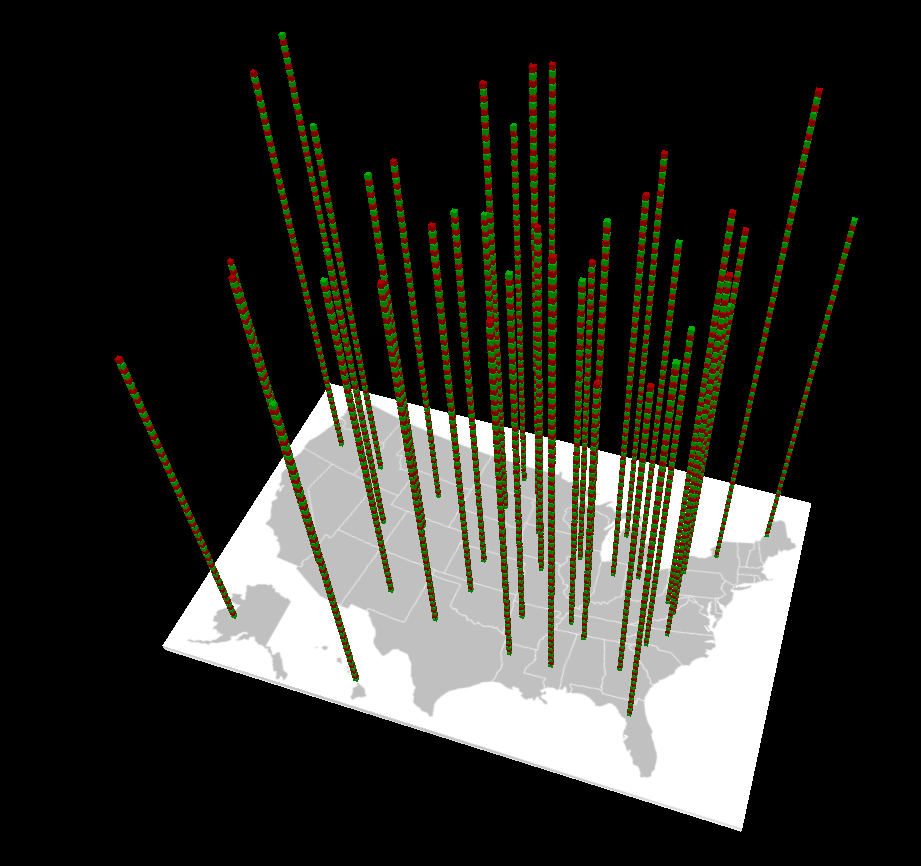
\includegraphics[width=\linewidth]{figures/viz3.PNG}
  \caption{Static visualization of message objects in time and space. Each column corresponds with the US state it stands on and goes forward in time from the bottom up. Therefore, each cube is a message in time and space.}
  \label{fig:viz2}
\end{figure}
After all the \emph{messageObjects} are visualized in this manner, we want to also show relationships between messages, to make it easier for the user, to follow conversational threads. After the user selects any \emph{messageObjects} he wants to understand more context of, we show the stream of conversation via arrows. If a post was done as a \emph{retweet} to another \emph{tweet}, an arrow is drawn from the cube, which represents the \emph{retweet}, to the one representing the original \emph{tweet}. This way the thread, which lead to the selected message, is opened up and can be analyzed by the user. An example for such a thread can be found at \ref{fig:viz4}.

\begin{figure}
  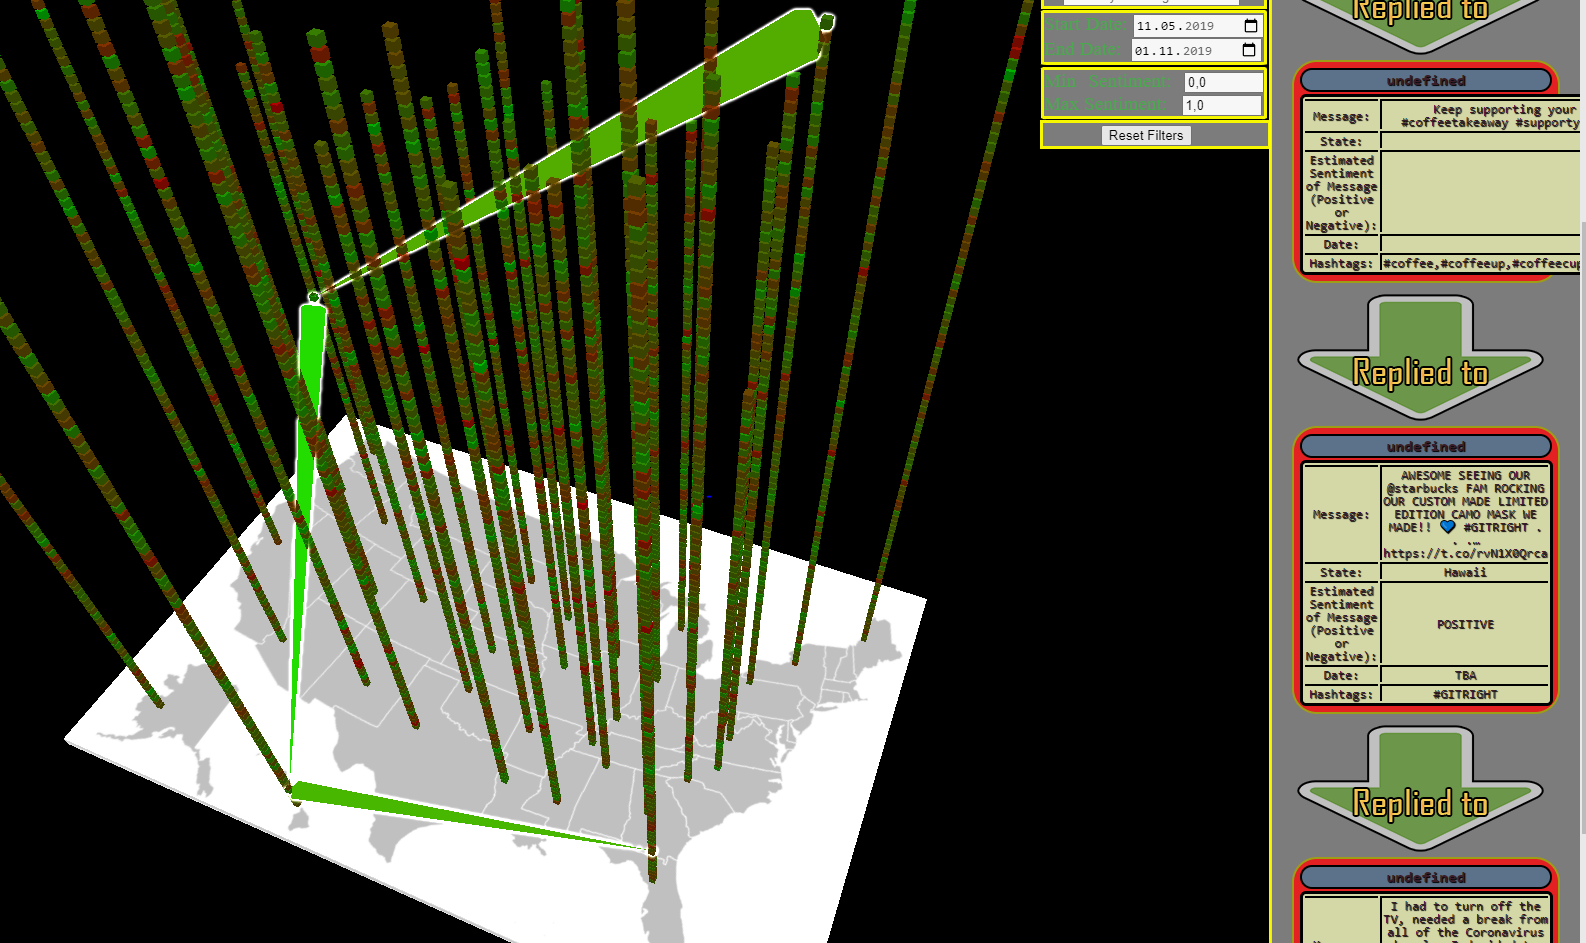
\includegraphics[width=\linewidth]{figures/example3.PNG}
  \caption{A typical conversational thread. The thread starts at the topmost cube and from there runs through arrows, which point from one message, to the message it is an answer to. The color of the arrow corresponds with the sentiment of the message, where green is positive and red is negative}
  \label{fig:viz4}
\end{figure}

\section{Filter}
To ensure that users may use the visualization, to answer specific research questions, we included the option to filter for individual criteria. Options for filtering include as follows:
\begin{itemize}
    \item Range of specific dates
    \item Range of sentiment values
    \item Inclusion of specific hashtags
    \item Exclusion of specific hashtags
\end{itemize}
This list is comprehensive of all possible options, and we strongly encourage the usage and inclusion of further possible filters, as more dimensions will be added to the visualization.
\section{Aggregate Visualization}
The basic 3D-rendering visualizes individual posts in a microblogging service and the relationship between them. It allows following conversational threads and not to get lost in a largely expanding conversational tree. However, broad overviews over different statistics can still be useful, when analyzing topics at hand. For this, we integrated a view with aggregated statistics over all available dimensions, which is visible in parallel to the rendering. An example for this view can be seen in \ref{fig:viz3}.
\begin{figure}
  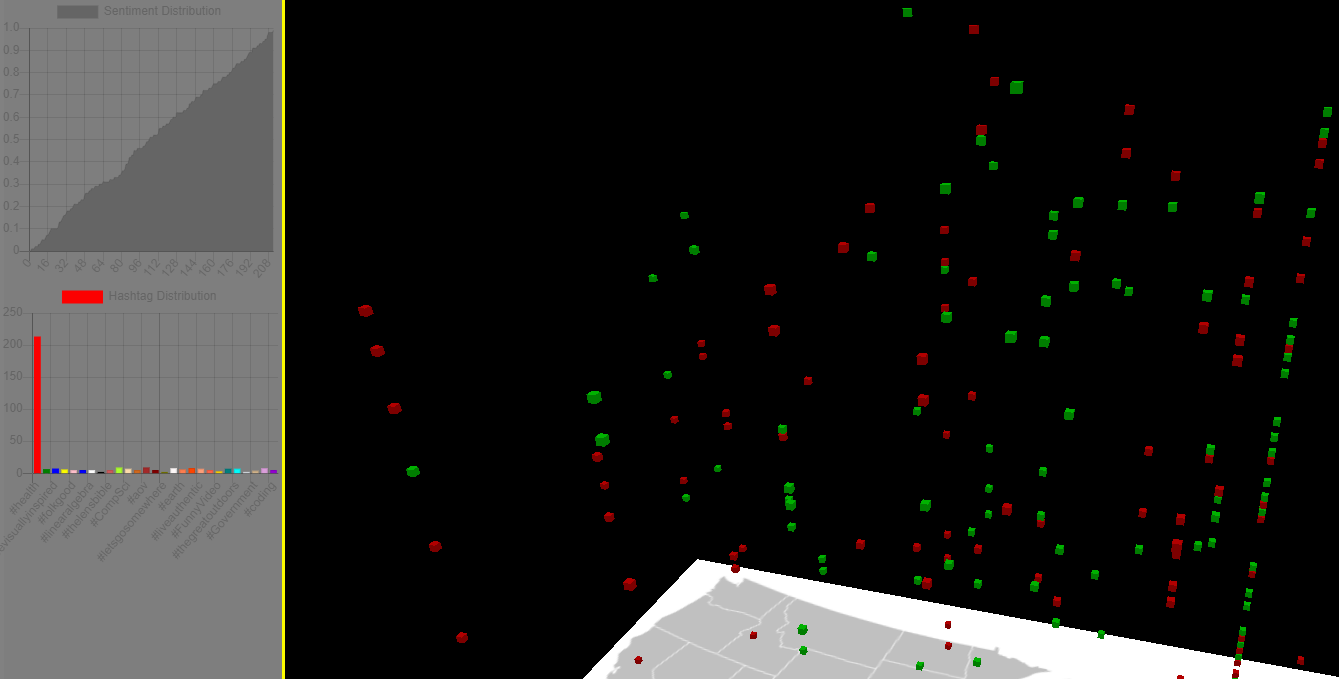
\includegraphics[width=\linewidth]{figures/stats.PNG}
  \caption{Rendering with statistics and filters applied. Only cubes are rendered, which do meet the requirements set by the filter. On the left, statistics over the sum of all rendered messages are shown.}
  \label{fig:viz3}
\end{figure}

This brings with it a few advantages. Firstly, it allows for more precise selection of filters, since one can directly see the effects which occur, when applying changes to any dimension. It also allows seeing a clearer picture of the discourse overall, contextualizing any single conversational thread, one is studying at the moment.